\section{Discussion} \label{sec:Discussion}
\subsection{Caveats}
This work and its results cannot be blindly trusted. There are a few assumptions and problems in the course of the investigations which might have influenced the results.
\textbf{GC selection}
One of the main problems in the analysis is the \acp{GC} selection. We applied a very simple recipe which only excluded \acp{GC} which were in a snapshot in a regime where the disk forces were very strong and should have destroyed the \ac{GC}. When selecting only a subset of the \acp{GC}, we have very different statistics of each progenitor group, e.g. the means shift significantly. A proper, physical selection would make these results more reliable. 
\textbf{Potential fit}
As we have discussed in Section \ref{subsec:wrong_pot_fit}, there are a few problems with the potential fit. The decomposition probably underestimates but also flares out the disk. For each component, the model differs from the data especially in the center. This is due to the choice of binning the data, fitting routines, etc. In total, the potential is good enough for the course of our investigations but, as one of the next steps, should be improved.
\textbf{Cold vs hot streams}
The assumption that the \ac{DF} of the \acp{GC} is a $\delta$-function requires them to be like a cold stream. Already in the introduction we have mentioned, that \ac{DG} mergers usually create hot streams so our \acp{GC} are probably dynamically hot and have a different, more complex \ac{DF}.
\textbf{}
\subsection{Comparison to observations}

\textbf{Excursion: coordinate transformations}
private communication with Wilma Trick
\textbf{\textit{Gaia}-Enceladus} \cite{Enceladus....Helmi...2018}
sagitarius modellierung single orbit Beispiel
-> zeigen dass kein single orbit ist (literatursuche)

\begin{figure}[htbp]
    \centering
    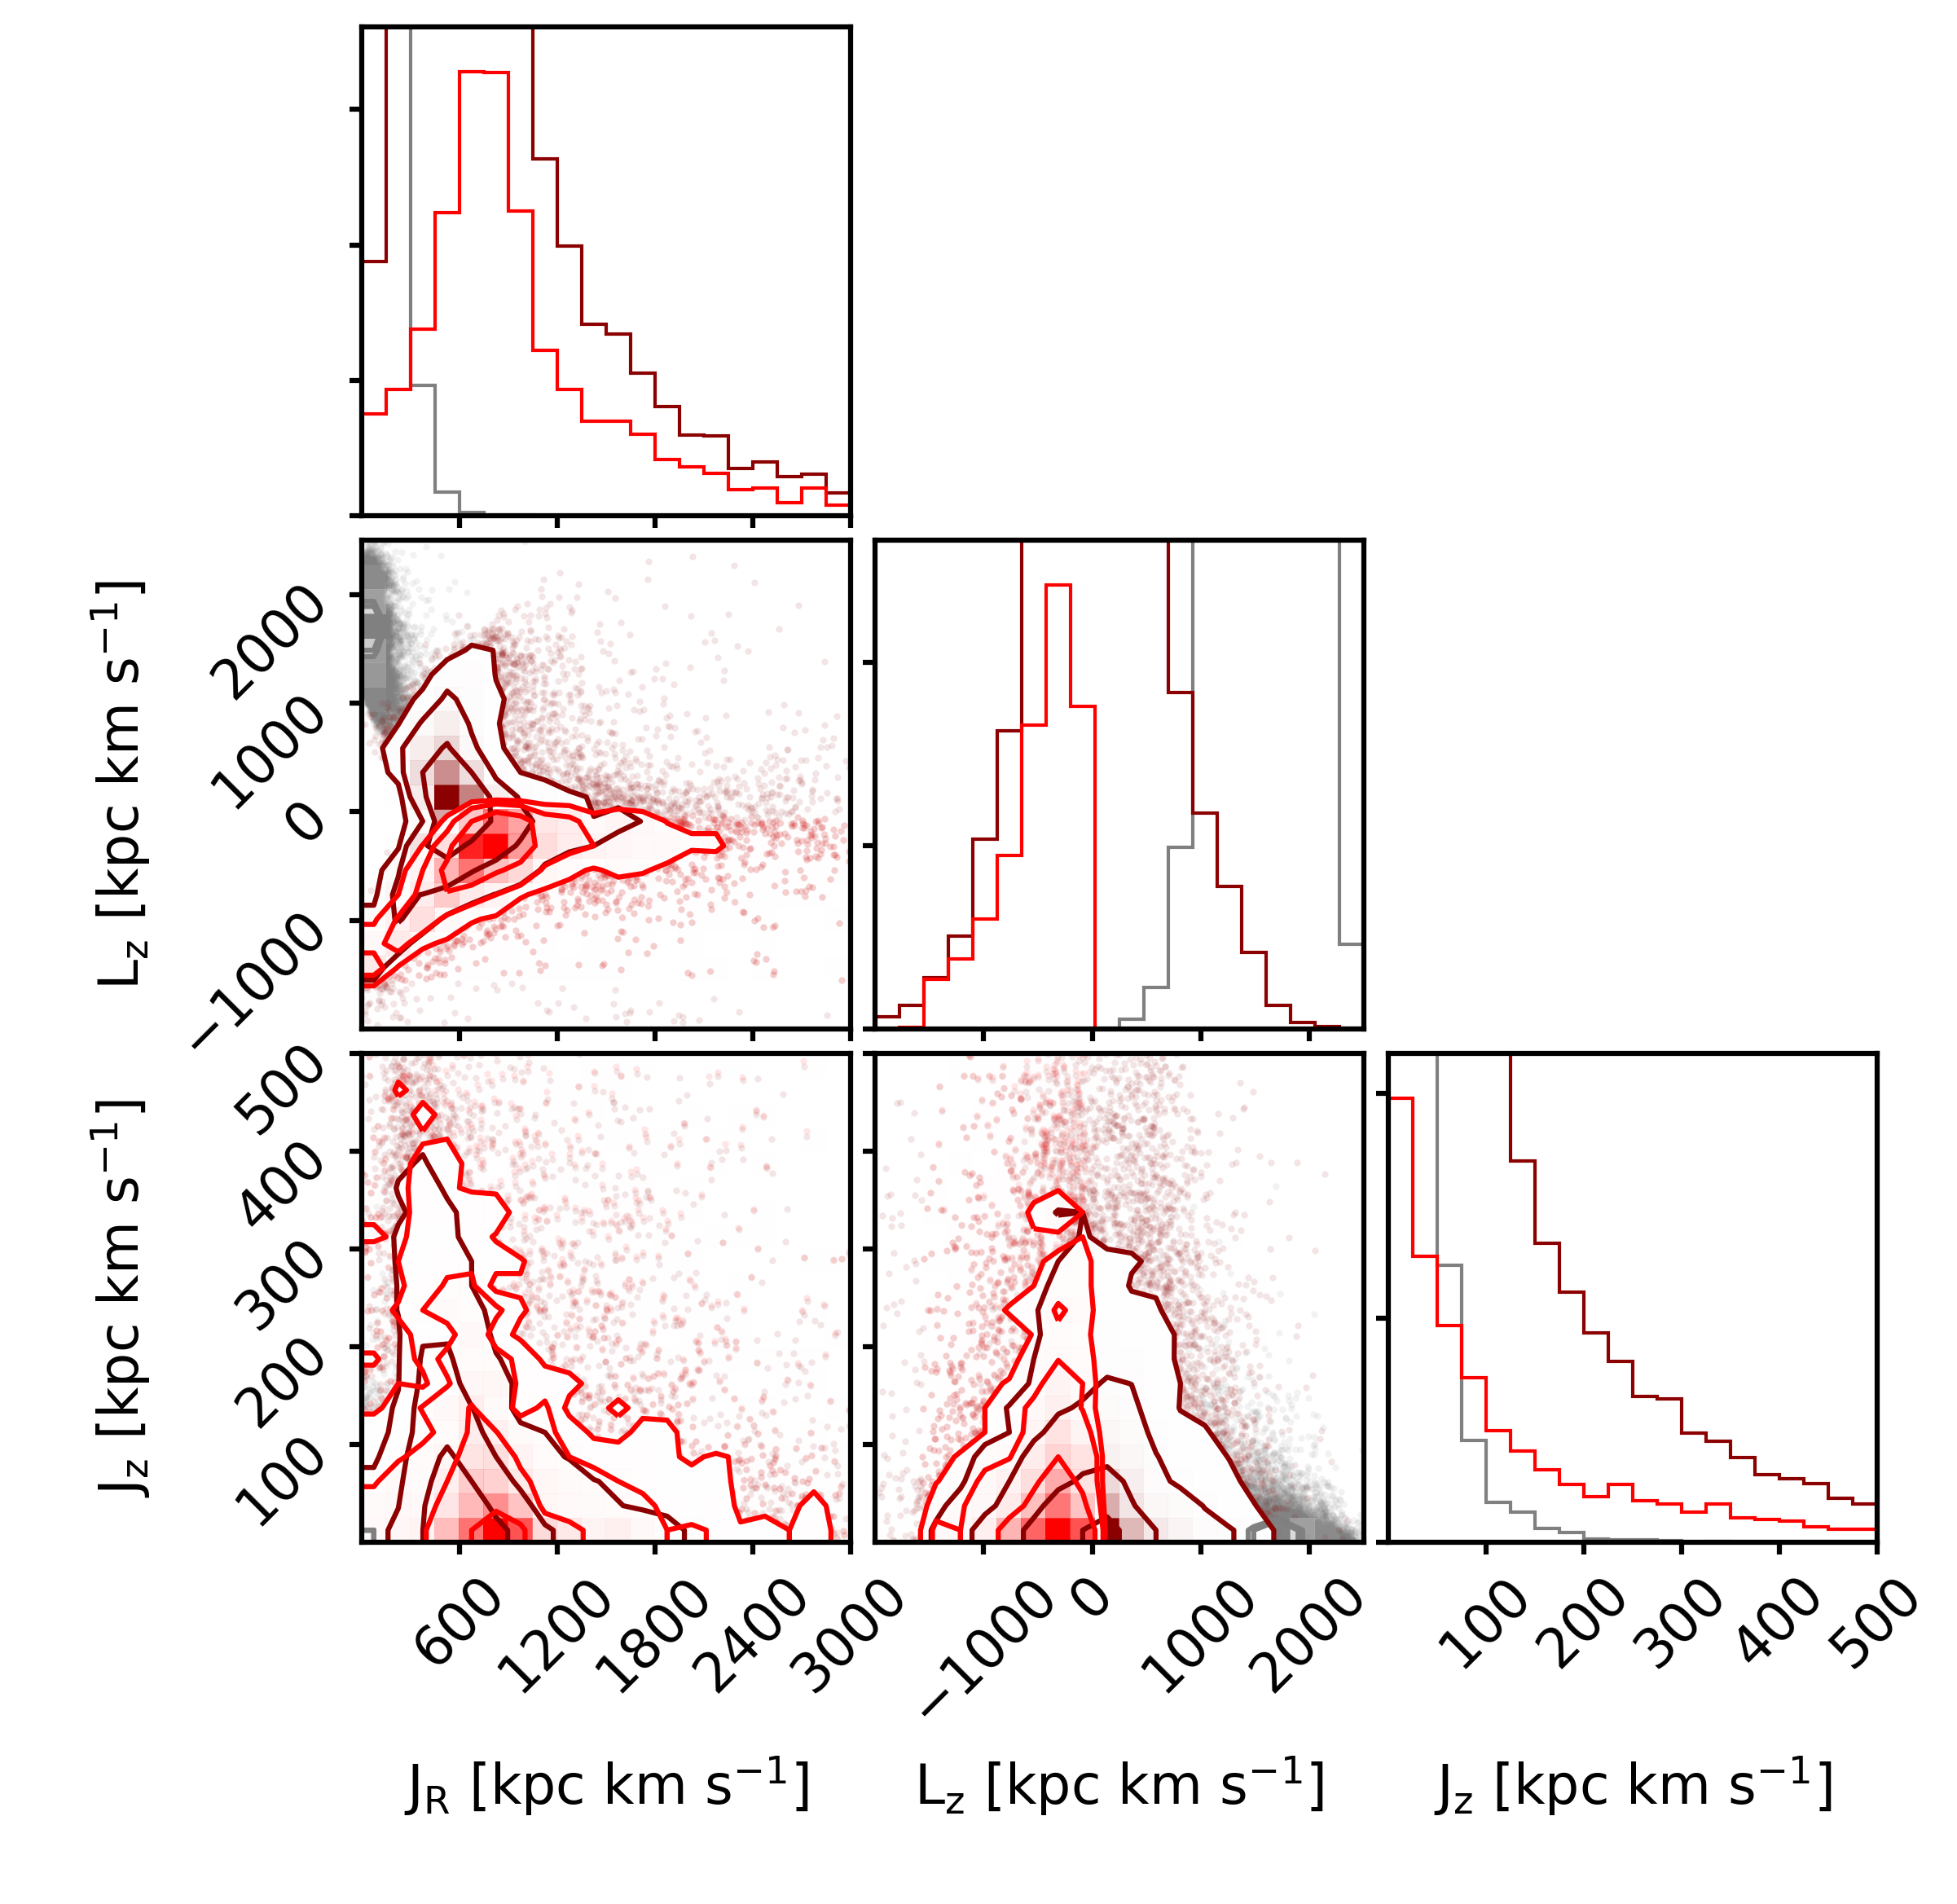
\includegraphics[width=1.0\textwidth]{plots/Discussion/Gaia_all_actions_MW14_talk3.png}
    \caption{\textit{Gaia}-Enceladus in action space in the MW14Potential.}
    \label{fig:act_both_merg_best_pot}
\end{figure}
\textbf{Andromeda?}

\subsection{Comparison to literature and other work}
\textbf{\acp{GC} formation in cosmological simulations} Timo Halbesma (PhD student at the MPA) is working on extracting \acp{GC} in the Auriga simulations which have proper physical properties and reasons to exist. Doing the same analysis with a set of proper \acp{GC} could change our results drastically. One reason could be that our population samples are too big and another one could be that if we select properly surviving \acp{GC} they could clump in action space because their orbits might stay constant and be properly affected by potential changes.\\
The E-MOSAICS simulation suite \citep{Pfeffer...E-MOSAICS...2018, Kruijssen...E-MOSAICS.MW..2018} are zoom-in simulations of the cosmological EAGLE \citep{Schaye...EAGLE...2015} simulations which have implemented models describing the formation, evolution, and disruption of star clusters. In these simulations, Meghan Hughes (PhD student at ESO/LJMU) works on modelling the potential and Sebastian Trujillo-Gomez (Post-doc at ARI) investigates the action of the \acp{GC}. 
\\\\
\textbf{Constraining gravitational potential}
There are attempts of applying adaptive dynamics to the \ac{MW}.
\begin{itemize}
    \item \textbf{\acp{DF} of \acp{GC}} \citep{Posti...MWmassGCs...2018}
    looked at all GCs and did not differentiate bw in-situ/ex-situ and coming from differetn \acp{DG}
    \item \textbf{Sharpen stellar streams in sims to find true potential} \citep{Sanderson...gravpotstreams...2017}
\end{itemize}


\subsection{Future Work}
\begin{itemize}
    \item richtige verteilunggsfunktion fuer accreted teilchen zu bestimmen 
    \item galpuy and AGAMA can calculate actions for N-body sims directly w/o need of gravitational potential - did not work yet because of technical issues -; test if action distribution and evolution behaves as we measured because of their nature and their physical evolution in the sim or because a analytic axisymmetric potential (in general or only our fit) comes not close to reality and messes these things up.
    \item 
\end{itemize}

